\section{\Grappa Overview}

\Grappa leverages as much freely available and commodity infrastructure as
possible. We use unmodified Linux for the operating system and an
off-the-shelf user-mode InfiniBand device driver stack~\cite{OFED}. MPI is
used for process setup and tear down. GASNet~\cite{gasnet} is used as the
underlying mechanism for remote memory reads and writes using active message
invocations. To this infrastructure, \Grappa adds  three main software components, shown in Figure~\ref{fig:grappa}:

\begin{figure}[t]
\begin{center}
  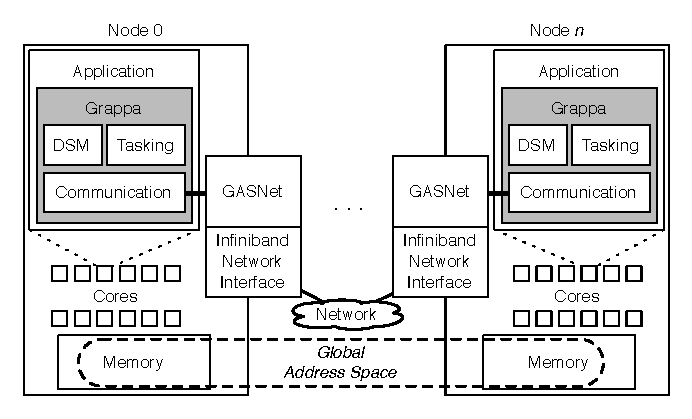
\includegraphics[width=0.95\columnwidth]{figs/system-overview}
\begin{minipage}{0.95\columnwidth}
  \caption{\label{fig:grappa} \Grappa system overview}
\end{minipage}
\vspace{-3ex}
\end{center}
\end{figure}

\begin{description}

\item [Tasking system.] The tasking system supports lightweight multithreading
to tolerate communication latency and global distributed work-stealing (i.e.,
tasks can be stolen from any node in the system), which provides automated
load balancing. The scheduler oversubscribes to have more worker threads than
required for latency tolerance. By having at least four workers per processor
core ready to run at all times, the scheduler can prefetch a worker's state
into cache to lower the likelihood of costly main memory accesses during a
context switch.

\item[Distributed shared memory.] The DSM system provides fine-grain access to
data anywhere in the system. It supports normal access operations such as
\emph{read\/} and \emph{write\/} as well as synchronizing operations such as
\emph{fetch-and-add\/}~\cite{fetchandadd}. It also offers explicit local
caching of any memory in the system, and delegates that directly operate on
remote data. The memory model offered is similar to what underpins
C/C++~\cite{N2480,N2800}, so it is familiar to programmers. The DSM system
design relies on the lightweight tasking system and communication layer in
order to offer high aggregate random access bandwidth for accessing remote
data.

\item[Communication layer.] The main goal of our communication layer is to
aggregate small messages into large ones, invisible to the application
programmer. Its interface is based on active messages~\cite{vonEicken92}.
Since aggregation and deaggregation of messages needs to be very efficient, we
made it highly concurrent with careful use of lock-free synchronization
operations.

\end{description}
